% Options for packages loaded elsewhere
\PassOptionsToPackage{unicode}{hyperref}
\PassOptionsToPackage{hyphens}{url}
%
\documentclass[
]{article}
\usepackage{amsmath,amssymb}
\usepackage{lmodern}
\usepackage{iftex}
\ifPDFTeX
  \usepackage[T1]{fontenc}
  \usepackage[utf8]{inputenc}
  \usepackage{textcomp} % provide euro and other symbols
\else % if luatex or xetex
  \usepackage{unicode-math}
  \defaultfontfeatures{Scale=MatchLowercase}
  \defaultfontfeatures[\rmfamily]{Ligatures=TeX,Scale=1}
\fi
% Use upquote if available, for straight quotes in verbatim environments
\IfFileExists{upquote.sty}{\usepackage{upquote}}{}
\IfFileExists{microtype.sty}{% use microtype if available
  \usepackage[]{microtype}
  \UseMicrotypeSet[protrusion]{basicmath} % disable protrusion for tt fonts
}{}
\makeatletter
\@ifundefined{KOMAClassName}{% if non-KOMA class
  \IfFileExists{parskip.sty}{%
    \usepackage{parskip}
  }{% else
    \setlength{\parindent}{0pt}
    \setlength{\parskip}{6pt plus 2pt minus 1pt}}
}{% if KOMA class
  \KOMAoptions{parskip=half}}
\makeatother
\usepackage{xcolor}
\usepackage[margin=1in]{geometry}
\usepackage{color}
\usepackage{fancyvrb}
\newcommand{\VerbBar}{|}
\newcommand{\VERB}{\Verb[commandchars=\\\{\}]}
\DefineVerbatimEnvironment{Highlighting}{Verbatim}{commandchars=\\\{\}}
% Add ',fontsize=\small' for more characters per line
\usepackage{framed}
\definecolor{shadecolor}{RGB}{248,248,248}
\newenvironment{Shaded}{\begin{snugshade}}{\end{snugshade}}
\newcommand{\AlertTok}[1]{\textcolor[rgb]{0.94,0.16,0.16}{#1}}
\newcommand{\AnnotationTok}[1]{\textcolor[rgb]{0.56,0.35,0.01}{\textbf{\textit{#1}}}}
\newcommand{\AttributeTok}[1]{\textcolor[rgb]{0.77,0.63,0.00}{#1}}
\newcommand{\BaseNTok}[1]{\textcolor[rgb]{0.00,0.00,0.81}{#1}}
\newcommand{\BuiltInTok}[1]{#1}
\newcommand{\CharTok}[1]{\textcolor[rgb]{0.31,0.60,0.02}{#1}}
\newcommand{\CommentTok}[1]{\textcolor[rgb]{0.56,0.35,0.01}{\textit{#1}}}
\newcommand{\CommentVarTok}[1]{\textcolor[rgb]{0.56,0.35,0.01}{\textbf{\textit{#1}}}}
\newcommand{\ConstantTok}[1]{\textcolor[rgb]{0.00,0.00,0.00}{#1}}
\newcommand{\ControlFlowTok}[1]{\textcolor[rgb]{0.13,0.29,0.53}{\textbf{#1}}}
\newcommand{\DataTypeTok}[1]{\textcolor[rgb]{0.13,0.29,0.53}{#1}}
\newcommand{\DecValTok}[1]{\textcolor[rgb]{0.00,0.00,0.81}{#1}}
\newcommand{\DocumentationTok}[1]{\textcolor[rgb]{0.56,0.35,0.01}{\textbf{\textit{#1}}}}
\newcommand{\ErrorTok}[1]{\textcolor[rgb]{0.64,0.00,0.00}{\textbf{#1}}}
\newcommand{\ExtensionTok}[1]{#1}
\newcommand{\FloatTok}[1]{\textcolor[rgb]{0.00,0.00,0.81}{#1}}
\newcommand{\FunctionTok}[1]{\textcolor[rgb]{0.00,0.00,0.00}{#1}}
\newcommand{\ImportTok}[1]{#1}
\newcommand{\InformationTok}[1]{\textcolor[rgb]{0.56,0.35,0.01}{\textbf{\textit{#1}}}}
\newcommand{\KeywordTok}[1]{\textcolor[rgb]{0.13,0.29,0.53}{\textbf{#1}}}
\newcommand{\NormalTok}[1]{#1}
\newcommand{\OperatorTok}[1]{\textcolor[rgb]{0.81,0.36,0.00}{\textbf{#1}}}
\newcommand{\OtherTok}[1]{\textcolor[rgb]{0.56,0.35,0.01}{#1}}
\newcommand{\PreprocessorTok}[1]{\textcolor[rgb]{0.56,0.35,0.01}{\textit{#1}}}
\newcommand{\RegionMarkerTok}[1]{#1}
\newcommand{\SpecialCharTok}[1]{\textcolor[rgb]{0.00,0.00,0.00}{#1}}
\newcommand{\SpecialStringTok}[1]{\textcolor[rgb]{0.31,0.60,0.02}{#1}}
\newcommand{\StringTok}[1]{\textcolor[rgb]{0.31,0.60,0.02}{#1}}
\newcommand{\VariableTok}[1]{\textcolor[rgb]{0.00,0.00,0.00}{#1}}
\newcommand{\VerbatimStringTok}[1]{\textcolor[rgb]{0.31,0.60,0.02}{#1}}
\newcommand{\WarningTok}[1]{\textcolor[rgb]{0.56,0.35,0.01}{\textbf{\textit{#1}}}}
\usepackage{graphicx}
\makeatletter
\def\maxwidth{\ifdim\Gin@nat@width>\linewidth\linewidth\else\Gin@nat@width\fi}
\def\maxheight{\ifdim\Gin@nat@height>\textheight\textheight\else\Gin@nat@height\fi}
\makeatother
% Scale images if necessary, so that they will not overflow the page
% margins by default, and it is still possible to overwrite the defaults
% using explicit options in \includegraphics[width, height, ...]{}
\setkeys{Gin}{width=\maxwidth,height=\maxheight,keepaspectratio}
% Set default figure placement to htbp
\makeatletter
\def\fps@figure{htbp}
\makeatother
\setlength{\emergencystretch}{3em} % prevent overfull lines
\providecommand{\tightlist}{%
  \setlength{\itemsep}{0pt}\setlength{\parskip}{0pt}}
\setcounter{secnumdepth}{-\maxdimen} % remove section numbering
\ifLuaTeX
  \usepackage{selnolig}  % disable illegal ligatures
\fi
\IfFileExists{bookmark.sty}{\usepackage{bookmark}}{\usepackage{hyperref}}
\IfFileExists{xurl.sty}{\usepackage{xurl}}{} % add URL line breaks if available
\urlstyle{same} % disable monospaced font for URLs
\hypersetup{
  pdftitle={HW2\_ISYE6414\_ashish\_dhiman},
  pdfauthor={Ashish Dhiman \textbar{} adhiman9@gatech.edu},
  hidelinks,
  pdfcreator={LaTeX via pandoc}}

\title{HW2\_ISYE6414\_ashish\_dhiman}
\author{Ashish Dhiman \textbar{}
\href{mailto:adhiman9@gatech.edu}{\nolinkurl{adhiman9@gatech.edu}}}
\date{2022-09-04}

\begin{document}
\maketitle

\begin{Shaded}
\begin{Highlighting}[]
\FunctionTok{library}\NormalTok{(ggplot2)}
\end{Highlighting}
\end{Shaded}

\hypertarget{part-1}{%
\section{Part 1}\label{part-1}}

\hypertarget{read-data-and-summary}{%
\subsection{Read Data and Summary}\label{read-data-and-summary}}

\begin{Shaded}
\begin{Highlighting}[]
\FunctionTok{head} \AttributeTok{{-}5}\NormalTok{ ./6414\textbackslash{}{-}HW2\textbackslash{}{-}taxes.csv}
\end{Highlighting}
\end{Shaded}

\begin{verbatim}
## "The following data are sale price, y ($10,000) and taxes, x ($10,000). ",
## Sale Price,Taxes
## 25.9,4.9176
## 29.5,5.0208
## 27.9,4.5429
\end{verbatim}

Since the first line does not have data we should skip it, also both the
data columns are in 10k USD scale.

\begin{Shaded}
\begin{Highlighting}[]
\NormalTok{df\_tax }\OtherTok{=} \FunctionTok{read.table}\NormalTok{(}\AttributeTok{file =}\StringTok{"./6414{-}HW2{-}taxes.csv"}\NormalTok{,}\AttributeTok{skip=}\DecValTok{1}\NormalTok{, }\AttributeTok{sep=}\StringTok{","}\NormalTok{,}\AttributeTok{header=}\ConstantTok{TRUE}\NormalTok{)}
\FunctionTok{head}\NormalTok{(df\_tax)}
\end{Highlighting}
\end{Shaded}

\begin{verbatim}
##   Sale.Price  Taxes
## 1       25.9 4.9176
## 2       29.5 5.0208
## 3       27.9 4.5429
## 4       25.9 4.5573
## 5       29.9 5.0597
## 6       29.9 3.8910
\end{verbatim}

\begin{Shaded}
\begin{Highlighting}[]
\FunctionTok{dim}\NormalTok{(df\_tax)}
\end{Highlighting}
\end{Shaded}

\begin{verbatim}
## [1] 26  2
\end{verbatim}

\begin{Shaded}
\begin{Highlighting}[]
\FunctionTok{summary}\NormalTok{(df\_tax)}
\end{Highlighting}
\end{Shaded}

\begin{verbatim}
##    Sale.Price        Taxes      
##  Min.   :25.90   Min.   :3.891  
##  1st Qu.:29.90   1st Qu.:5.057  
##  Median :33.70   Median :5.974  
##  Mean   :34.61   Mean   :6.405  
##  3rd Qu.:38.15   3rd Qu.:7.873  
##  Max.   :45.80   Max.   :9.142  
##  NA's   :2       NA's   :2
\end{verbatim}

\begin{Shaded}
\begin{Highlighting}[]
\NormalTok{df\_tax }\OtherTok{=}\NormalTok{ df\_tax[}\DecValTok{1}\SpecialCharTok{:}\NormalTok{(}\FunctionTok{nrow}\NormalTok{(df\_tax)}\SpecialCharTok{{-}}\DecValTok{2}\NormalTok{),] }\CommentTok{\#Remove last two empty rows}
\FunctionTok{dim}\NormalTok{(df\_tax)}
\end{Highlighting}
\end{Shaded}

\begin{verbatim}
## [1] 24  2
\end{verbatim}

\hypertarget{question-1-scatter-plot}{%
\subsection{Question 1: Scatter Plot}\label{question-1-scatter-plot}}

\begin{Shaded}
\begin{Highlighting}[]
\NormalTok{title\_i }\OtherTok{=} \StringTok{"Sales Price vs Annual Taxes (both in 10k USD)"}
\FunctionTok{plot}\NormalTok{(}\AttributeTok{x=}\NormalTok{df\_tax}\SpecialCharTok{$}\NormalTok{Taxes, }\AttributeTok{y=}\NormalTok{df\_tax}\SpecialCharTok{$}\NormalTok{Sale.Price, }\AttributeTok{type =}\StringTok{"p"}\NormalTok{,}\AttributeTok{main =}\NormalTok{ title\_i)}
\end{Highlighting}
\end{Shaded}

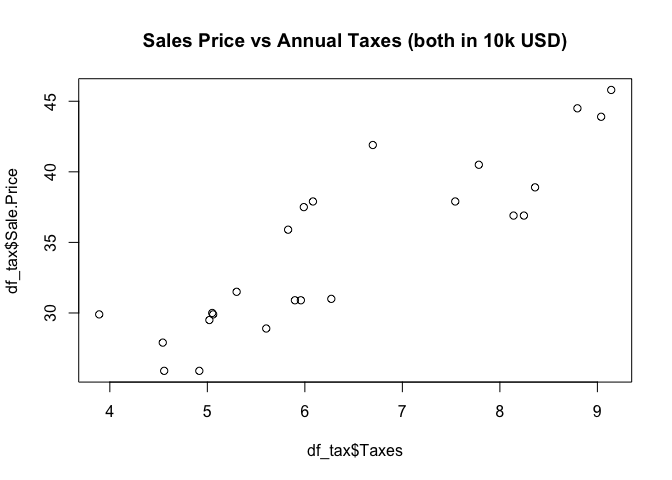
\includegraphics{hw2_6414_ashish_dhiman_files/figure-latex/unnamed-chunk-5-1.pdf}

\(\color{blue}{\text{From the above plot, a linear realationship between Sales Price and Taxes is apparent.}}\)

\(\color{blue}{\text{The strength of the linear realtionship can also be tested with corealtion between x and y.}}\)

\begin{Shaded}
\begin{Highlighting}[]
\FunctionTok{print}\NormalTok{ (}\FunctionTok{paste}\NormalTok{(}\StringTok{"Corealtion on full data:"}\NormalTok{,}\FunctionTok{round}\NormalTok{(}\FunctionTok{cor}\NormalTok{(df\_tax}\SpecialCharTok{$}\NormalTok{Taxes,df\_tax}\SpecialCharTok{$}\NormalTok{Sale.Price),}\DecValTok{2}\NormalTok{)))}
\end{Highlighting}
\end{Shaded}

\begin{verbatim}
## [1] "Corealtion on full data: 0.88"
\end{verbatim}

\(\color{blue}{\text{A corelation of 0.88 is pretty significant and supports strong linear realtionship between x and y.}}\)

\hypertarget{question-2-fit-slr}{%
\subsection{Question 2: Fit SLR}\label{question-2-fit-slr}}

\begin{Shaded}
\begin{Highlighting}[]
\CommentTok{\#Fit SLR}
\NormalTok{model0 }\OtherTok{\textless{}{-}} \FunctionTok{lm}\NormalTok{(Sale.Price }\SpecialCharTok{\textasciitilde{}}\NormalTok{ Taxes, }\AttributeTok{data =}\NormalTok{ df\_tax)}
\NormalTok{model0}
\end{Highlighting}
\end{Shaded}

\begin{verbatim}
## 
## Call:
## lm(formula = Sale.Price ~ Taxes, data = df_tax)
## 
## Coefficients:
## (Intercept)        Taxes  
##      13.320        3.324
\end{verbatim}

\begin{Shaded}
\begin{Highlighting}[]
\CommentTok{\#Superpositioning regression line on }
\FunctionTok{ggplot}\NormalTok{(df\_tax, }\FunctionTok{aes}\NormalTok{(Taxes, Sale.Price)) }\SpecialCharTok{+} \CommentTok{\#aes(x,y)}
  \FunctionTok{geom\_point}\NormalTok{() }\SpecialCharTok{+}
  \FunctionTok{stat\_smooth}\NormalTok{(}\AttributeTok{method =}\NormalTok{ lm, }\AttributeTok{se =} \ConstantTok{FALSE}\NormalTok{)}
\end{Highlighting}
\end{Shaded}

\begin{verbatim}
## `geom_smooth()` using formula 'y ~ x'
\end{verbatim}

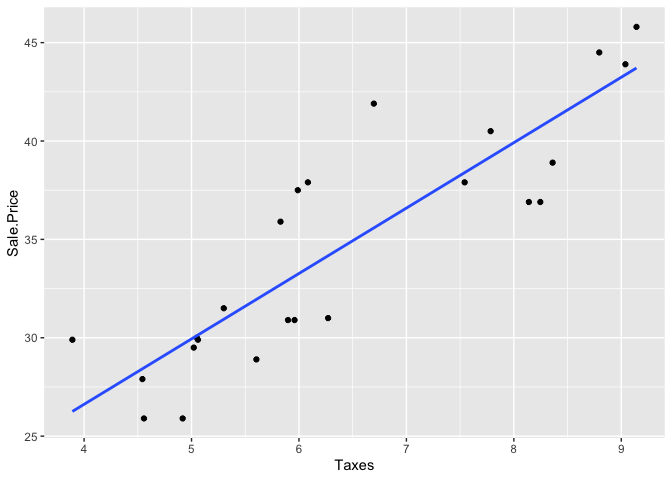
\includegraphics{hw2_6414_ashish_dhiman_files/figure-latex/unnamed-chunk-7-1.pdf}

\[
From\ above, we\ have:\\
\] \[
\hat{\beta}_0:= Intecept = 13.320,\\
\] \[
\hat{\beta}_1:=Slope = 3.324,\ and\\
\] \[
\hat{y} = \hat{\beta}_0 +\hat{\beta}_1 * x = 13.320 + 3.324 *x
\]

\hypertarget{question-3-meaning-of-beta1-hatbeta_1}{%
\subsection{\texorpdfstring{Question 3: Meaning of beta1
(\(\hat{\beta}_1\)):}{Question 3: Meaning of beta1 (\textbackslash hat\{\textbackslash beta\}\_1):}}\label{question-3-meaning-of-beta1-hatbeta_1}}

\(\hat{\beta}_1\) implies the slope of the SLR line we have fit to the
data. In other words, it tells us, the change recorded in y (on average)
for every one unit of change in x.

\(\color{blue}{\text{In this case, this implies for every 10k USD change in Taxes, the Price goies up by 3,324 USD (on average).}}\)

\hypertarget{question-4-meaning-of-beta0-hatbeta_0}{%
\subsection{\texorpdfstring{Question 4: Meaning of beta0
(\(\hat{\beta}_0\)):}{Question 4: Meaning of beta0 (\textbackslash hat\{\textbackslash beta\}\_0):}}\label{question-4-meaning-of-beta0-hatbeta_0}}

\(\hat{\beta}_0\) implies the predicted value of y given x is zero.

\(\color{blue}{\text{In this case, this implies for 0 USD in taxes (let's assume), the the expected prices is 13,320 USD}}.\)

\(\color{blue}{\text{This case is improbable but still possible, and would imply that the state has relaxed the tax rate to 0%}}.
\)

This could be done by state to foster investment my individuals and
firms.

\hypertarget{question-5-value-of-s-s2-and-sse}{%
\subsection{\texorpdfstring{Question 5: value of s, \(s^2\) and
SSE:}{Question 5: value of s, s\^{}2 and SSE:}}\label{question-5-value-of-s-s2-and-sse}}

s and s\^{}2

\begin{Shaded}
\begin{Highlighting}[]
\NormalTok{s\_squared }\OtherTok{=} \FunctionTok{sum}\NormalTok{(}\FunctionTok{sapply}\NormalTok{(model0[}\StringTok{"residuals"}\NormalTok{], }\ControlFlowTok{function}\NormalTok{(x) x}\SpecialCharTok{\^{}}\DecValTok{2}\NormalTok{))}\SpecialCharTok{/}\NormalTok{(}\FunctionTok{nrow}\NormalTok{(df\_tax)}\SpecialCharTok{{-}}\DecValTok{2}\NormalTok{)}
\NormalTok{s\_squared}
\end{Highlighting}
\end{Shaded}

\begin{verbatim}
## [1] 8.767753
\end{verbatim}

\begin{Shaded}
\begin{Highlighting}[]
\NormalTok{s\_squared}\SpecialCharTok{\^{}}\FloatTok{0.5}
\end{Highlighting}
\end{Shaded}

\begin{verbatim}
## [1] 2.961039
\end{verbatim}

\hypertarget{sse-from-fitted-values}{%
\subsubsection{SSE from fitted values}\label{sse-from-fitted-values}}

\(SSE = \sum_{i \in all\ data\ points}([y_i - \hat{y}_i]^2)\)

\begin{Shaded}
\begin{Highlighting}[]
\NormalTok{y\_hat }\OtherTok{=} \FunctionTok{fitted}\NormalTok{(model0)}
\NormalTok{y\_act }\OtherTok{=}\NormalTok{ df\_tax}\SpecialCharTok{$}\NormalTok{Sale.Price}

\NormalTok{sse }\OtherTok{=} \FunctionTok{sum}\NormalTok{((y\_act }\SpecialCharTok{{-}}\NormalTok{ y\_hat)}\SpecialCharTok{\^{}}\DecValTok{2}\NormalTok{)}
\FunctionTok{print}\NormalTok{ (}\FunctionTok{paste}\NormalTok{(}\StringTok{"sse is"}\NormalTok{,sse))}
\end{Highlighting}
\end{Shaded}

\begin{verbatim}
## [1] "sse is 192.89056494381"
\end{verbatim}

\begin{Shaded}
\begin{Highlighting}[]
\NormalTok{sse}\SpecialCharTok{/}\NormalTok{(}\FunctionTok{nrow}\NormalTok{(df\_tax)}\SpecialCharTok{{-}}\DecValTok{2}\NormalTok{)}
\end{Highlighting}
\end{Shaded}

\begin{verbatim}
## [1] 8.767753
\end{verbatim}

\hypertarget{part-2}{%
\section{Part 2}\label{part-2}}

\hypertarget{question-6-least-square-estimate-of-beta0-beta1}{%
\subsection{Question 6: Least Square Estimate of beta0,
beta1:}\label{question-6-least-square-estimate-of-beta0-beta1}}

\[
\hat{\beta}_1 = \frac{(\sum_i{x_iy_i}) - n\overline{x}\overline{y}}{\sum_i{{x_i}^2} - n\overline{x}^2},\\\]
\[
we\ have:\\
\] \[
\sum_i{x_iy_i} = 1697.8,\\\] \[
n\overline{x}\overline{y} = n * \frac{\sum_i{x_i}}{n} * \frac{\sum_i{y_i}}{n},\\\]
\[
\sum_i{{x_i}^2} = 157.42,\\\] \[
n\overline{x}^2 = n * \frac{\sum_i{x_i}}{n} = \sum_i{x_i} = 14*(43/14)^2
\]

\begin{Shaded}
\begin{Highlighting}[]
\NormalTok{num }\OtherTok{=} \FloatTok{1697.8} \SpecialCharTok{{-}}\NormalTok{ (}\DecValTok{14} \SpecialCharTok{*}\NormalTok{ (}\DecValTok{43}\SpecialCharTok{/}\DecValTok{14}\NormalTok{) }\SpecialCharTok{*}\NormalTok{ (}\DecValTok{572}\SpecialCharTok{/}\DecValTok{14}\NormalTok{))}
\NormalTok{num}
\end{Highlighting}
\end{Shaded}

\begin{verbatim}
## [1] -59.05714
\end{verbatim}

\begin{Shaded}
\begin{Highlighting}[]
\NormalTok{denom }\OtherTok{=} \FloatTok{157.42} \SpecialCharTok{{-}}\NormalTok{ (}\DecValTok{14}\SpecialCharTok{*}\NormalTok{(}\DecValTok{43}\SpecialCharTok{/}\DecValTok{14}\NormalTok{)}\SpecialCharTok{\^{}}\DecValTok{2}\NormalTok{)}
\NormalTok{denom}
\end{Highlighting}
\end{Shaded}

\begin{verbatim}
## [1] 25.34857
\end{verbatim}

\begin{Shaded}
\begin{Highlighting}[]
\NormalTok{beta1 }\OtherTok{=}\NormalTok{ num}\SpecialCharTok{/}\NormalTok{denom}
\FunctionTok{print}\NormalTok{ (}\FunctionTok{paste}\NormalTok{(}\StringTok{"Intecept (or beta0)"}\NormalTok{,beta1))}
\end{Highlighting}
\end{Shaded}

\begin{verbatim}
## [1] "Intecept (or beta0) -2.32980162308386"
\end{verbatim}

\[
\hat{\beta}_0 = \overline{y} - \hat{\beta}_1\overline{x}
\]

\begin{Shaded}
\begin{Highlighting}[]
\NormalTok{beta0 }\OtherTok{=}\NormalTok{ (}\DecValTok{572}\SpecialCharTok{/}\DecValTok{14}\NormalTok{) }\SpecialCharTok{{-}}\NormalTok{ beta1}\SpecialCharTok{*}\NormalTok{(}\DecValTok{43}\SpecialCharTok{/}\DecValTok{14}\NormalTok{)}
\FunctionTok{print}\NormalTok{ (}\FunctionTok{paste}\NormalTok{(}\StringTok{"Intecept (or beta0)"}\NormalTok{,beta0))}
\end{Highlighting}
\end{Shaded}

\begin{verbatim}
## [1] "Intecept (or beta0) 48.0129621280433"
\end{verbatim}

\hypertarget{question-7-calculate-sse}{%
\subsection{Question 7: Calculate SSE}\label{question-7-calculate-sse}}

\[
SSE = SS_{yy} - \hat{\beta}_1SS_{xy},\] \[
SS_{yy} = \sum_i{(y_i - \overline{y})^2} = \sum_i{y_i}^2 - n\overline{y}^2\]
\[
SS_{xy} = (\sum_i{x_iy_i}) - n\overline{x}\overline{y}
\]

\begin{Shaded}
\begin{Highlighting}[]
\NormalTok{SS\_yy }\OtherTok{=} \DecValTok{23530} \SpecialCharTok{{-}} \DecValTok{14} \SpecialCharTok{*}\NormalTok{((}\DecValTok{572}\SpecialCharTok{/}\DecValTok{14}\NormalTok{))}\SpecialCharTok{\^{}}\DecValTok{2}
\NormalTok{SS\_xy }\OtherTok{=}\NormalTok{ num }\CommentTok{\#from ques7}
\NormalTok{SSE }\OtherTok{=}\NormalTok{ SS\_yy }\SpecialCharTok{{-}}\NormalTok{ beta1 }\SpecialCharTok{*}\NormalTok{ SS\_xy}
\NormalTok{sigma2 }\OtherTok{=}\NormalTok{ SSE}\SpecialCharTok{/}\NormalTok{(}\DecValTok{14{-}2}\NormalTok{)}
\FunctionTok{print}\NormalTok{ (}\FunctionTok{paste}\NormalTok{(}\StringTok{"SSE is"}\NormalTok{,SSE))}
\end{Highlighting}
\end{Shaded}

\begin{verbatim}
## [1] "SSE is 22.1228584310236"
\end{verbatim}

\begin{Shaded}
\begin{Highlighting}[]
\FunctionTok{print}\NormalTok{ (}\FunctionTok{paste}\NormalTok{(}\StringTok{"Sigma squared is"}\NormalTok{,sigma2))}
\end{Highlighting}
\end{Shaded}

\begin{verbatim}
## [1] "Sigma squared is 1.84357153591864"
\end{verbatim}

\hypertarget{question-8-y-for-x-3.7}{%
\subsection{Question 8: y for x =3.7}\label{question-8-y-for-x-3.7}}

\begin{Shaded}
\begin{Highlighting}[]
\NormalTok{y\_act }\OtherTok{=} \FloatTok{46.1}
\NormalTok{y\_hat }\OtherTok{=}\NormalTok{ beta0 }\SpecialCharTok{+}\NormalTok{ beta1 }\SpecialCharTok{*} \FloatTok{3.7}
\NormalTok{residual }\OtherTok{=}\NormalTok{ y\_act }\SpecialCharTok{{-}}\NormalTok{ y\_hat}
\FunctionTok{print}\NormalTok{ (}\FunctionTok{paste}\NormalTok{(}\StringTok{"Predicted Y value is"}\NormalTok{,y\_hat))}
\end{Highlighting}
\end{Shaded}

\begin{verbatim}
## [1] "Predicted Y value is 39.392696122633"
\end{verbatim}

\begin{Shaded}
\begin{Highlighting}[]
\FunctionTok{print}\NormalTok{ (}\FunctionTok{paste}\NormalTok{(}\StringTok{"Corresponding Residual is"}\NormalTok{,residual))}
\end{Highlighting}
\end{Shaded}

\begin{verbatim}
## [1] "Corresponding Residual is 6.707303877367"
\end{verbatim}

\end{document}
